\chapter{Resultados y discusi\'on}
\label{ch:resAuger}

Una vez definidos los criterios de selección es posible calcular la exposición del detector y llevar a cabo la búsqueda de candidatos.



\section{C\'alculo de la exposici\'on}
\label{sc:expoNu}
	
	La exposición es una cantidad comunmente utilizada en física de astropartículas para caracterizar una medición.
	Se la define como la magnitud que, convolucionada con un flujo de partículas $\frac{dN_{\nu}}{d\Gamma}$, resulta en la cantidad de eventos que se espera haber detectado durante la misma, como se muestra en la ecuación \ref{eq:exp0}.
	%
	\begin{equation}
	 N_{esp}=\int\limits_{\Gamma}~\frac{dN_{\nu}}{d\Gamma}~\mathscr{E}(\Gamma) ~d\Gamma
	 \label{eq:exp0}
	\end{equation}
	%
	En esta, $\Gamma$ simboliza el conjunto de variables del que dependa la detección, que en este trabajo corresponde a $(E_{\nu},A,\Omega,T)$\footnote{Se desprecia cualquier tipo de inhomogeneidad en el flujo.}, es decir, la energía de los neutrinos incidentes, el área del detector, el ángulo sólido que se observa y el tiempo durante el que se mide, respectivamente.
	
	De la ecuación \ref{eq:exp0} se desprende entonces que, como $\frac{dN_{\nu}}{d\Gamma}$ es la cantidad de neutrinos de energía $E_{\nu}$ que alcanzan el detector por unidad de área, ángulo sólido y tiempo, la exposición debe representar qué cantidad de cada energía se espera haber detectado en promedio en cada unidad de área del detector y en cada instante de tiempo.
	Es decir, la exposición contiene toda la información correspondiente a la medición y al detector, mientras que el flujo incluye la física de la fuente de lo que se espera detectar.
	
	Si se considera a $\frac{dN_{\nu}}{d\Gamma}$ como un flujo difuso $\Phi(E_{\nu})$, es decir isótropo, homogeneo y constante en el tiempo, la ecuación \ref{eq:exp0} puede escribirse como \ref{eq:exp1}.
	%
	\begin{equation}
	 N_{esp}=\int\limits_{E_{\nu}}~\Phi(E_{\nu})\left[~\iiint\limits_{T~\Omega~A}\mathscr{E}(E_{\nu},A,\Omega,T) ~dA~d\Omega~dT~\right]~dE_\nu
	 \label{eq:exp1}
	\end{equation}
	%
	La función de $E_\nu$ entre corchetes, que corresponde a la exposición integrada en el caso de un flujo difuso, será llamada de aquí en más \emph{exposición del detector} y será simbolizada por la letra $\cal E$, como se muestra en la ecuación \ref{eq:exp2}.
	%
	\begin{equation}
	 {\cal E}(E_\nu)\equiv\iiint\limits_{T~\Omega~A}\mathscr{E}(E_{\nu},A,\Omega,T) ~dA~d\Omega~dT
	 \label{eq:exp2}
	\end{equation}
	%
	El objetivo a partir de aquí es la construcción de esta cantidad que requiere de los siguientes ingredientes:
	\begin{enumerate}
	 \item La probabilidad de que un neutrino de energía $E_\nu$ proveniente del sector $\Omega$~\footnote{Es decir, cuya dirección se caracteriza por los ángulos $(\theta,\phi)$.} de inicio a una lluvia atmosférica extendida de parámetros $X$.
	 \item La probabilidad de que una lluvia de parámetros $X$ dispare el detector y que el evento registrado sea identificado como un neutrino, es decir, las eficiencias de identificación.
	 \item La integración de estas probabilidades sobre el área del detector, el tiempo de medición, las diferentes direcciones de arrivo y las distintas lluvias atmosféricas que se puedan generar.
	\end{enumerate}
	
	Teniendo esto en cuenta, la ecuación \ref{eq:exp2} puede escribirse como en la ecuación \ref{eq:exp3}.
	%
	\begin{equation}
	 {\cal E}(E_\nu)\equiv\iiiint\limits_{T~\Omega~A~X}P(X|E_{\nu},A,\Omega,T)~\epsilon(X,E_{\nu},A,\Omega,T) ~dX~dA~d\Omega~dT
	 \label{eq:exp3}
	\end{equation}
	% 
	Según lo que se expuso en la sección \ref{sc:libGen} para eventos ES el parámetro $X$ debe corresponder al conjunto $(E_\tau,{\rm x_d})$, mientras que en el caso de DG corresponde a la profundidad inclinada de interacción $D$.
	Por otro lado, la probabilidad de ocurrencia de un evento de parámetros $X$ simplemente incluye la información del blanco con el que los neutrinos interactúan: la tierra en ES y la atmósfera en DG. 
	En ambos casos en este trabajo se desprecian las fluctuaciones que estos puedan tener durante el tiempo que dura la medición o al variar la fracción del detector que se esté estudiando, por lo que $P(X|E_{\nu},A,\Omega,T)~\rightarrow~P(X|E_{\nu},\Omega)$.
	Incuyendo toda esta información, para calcular la exposición del detector habrá que realizar las integrales de las ecuaciones \ref{eq:exp4DG} y \ref{eq:exp4ES}.
	%
	\begin{equation}
	 {\cal E}_{DG}(E_\nu)\equiv\iint\limits_{D~\Omega}P(D|E_{\nu},\Omega)~
	 \left[~
	 \iint\limits_{T~A}\epsilon(D,E_{\nu},A,\Omega,T)~dA~dT
	 \right]
	 ~d\Omega~dD
	 \label{eq:exp4DG}
	\end{equation}
	%
	\begin{equation}
	 {\cal E}_{ES}(E_\nu)\equiv\iiint\limits_{E_\tau~{\rm x_d}~\Omega}P({\rm x_d},E_\tau|E_{\nu},\Omega)~
	 \left[~
	 \iint\limits_{T~A}\epsilon({\rm x_d},E_\tau,A,\Omega,T)~dA~dT
	 \right]
	 ~d\Omega~d{\rm x_d}~dE_\tau
	 \label{eq:exp4ES}
	\end{equation}
	%
	
	En las siguientes secciones se abordará la obtención de cada uno de los términos.
	
	\subsection{Término de probabilidad}
	
	El término de probabilidad conecta el flujo con las eficiencias en el cálculo de la exposición.
	En este caso, el flujo representa la cantidad de eventos que se esperan por unidad de área, tiempo y ángulo sólido, mientras que por construcción las eficiencias corresponden a la cantidad de eventos detectados segun variables relacionadas con el proceso de medición\footnote{$(E_\tau,\Omega,{\rm x_d})$ en ES y $(E_\nu,\Omega,D)$ en DG.}.
	Entonces, coloquialmente este término responde a la prgunta: ¿cuántos de los eventos que predice el flujo espero en cada bin en que conozco la eficiencia?
	
	\subsubsection{Eventos DG}
	
	Como se expuso en la sección \ref{sbsc:easDG}, el camino libre medio de los neutrinos es varios órdenes de magnitud mayor que el espesor de la atmósfera, por lo que es una muy buena aproximacion considerar la probabilidad de interacción una constante para cualquier profundidad de interacción, o lo que es lo mismo, que la magnitud del flujo no depende de la misma.
	Con esto en mente, para obtener la expresión de $P(D|E_{\nu},\Omega)$ es útil primero considerar un caso simplificado: un haz de partículas, con flujo lineal~$F$ (medido en partículas por unidad de área por unidad de tiempo), que incide sobre un blanco con~$N$ elementos dispersores. En esta situación la cantidad de colisiones~$n$ por unidad de tiempo está dada por:
	%
	\begin{equation}
	% \frac{\Delta n}{\Delta t} 
	n = F\,\sigma\,N
	\end{equation}
	% 
	en donde $\sigma$ es la sección eficaz de interacción entre las partículas del haz y las del blanco.
	Si se considera un blanco de masa~$M$ formado por elementos dispersores de masa~$m$ el número de colisiones por unidad de tiempo es simplemente:
	%
	\begin{equation}
	% \frac{\Delta n}{\Delta t} 
	n = F\,\sigma\,\frac{M}{m}
	\end{equation}
	% 

	El resultado anterior se puede extender para analizar el caso de un flujo diferencial difuso~$\Phi(E_{\nu})$ y un detector plano que registra todas las lluvias producidas por neutrinos que satisfacen las siguientes condiciones  (ver figura \ref{fig:diferencialMasa}):
	%
	\begin{itemize}
	\item su dirección de arribo apunta a una región $\Delta A$ del detector ubicada en $\vec{r}$
	\item su dirección de arribo $(\theta,\phi)$ está en un rango 
	$\Delta \Omega=\sen\theta\,\Delta\theta\,\Delta\phi$
	\item su energía~$E_{\nu}$ está en un rango $\Delta E_{\nu}$
	\item interactúa a una profundidad másica~$D$ en el rango $[D, D+\Delta D]$. 
	\end{itemize}
	%
	En este caso el número de lluvias observadas por unidad de tiempo está dado por
	%
	\begin{equation}
	% \frac{\Delta \mathfrak{N}}{\Delta t}
	n = \Phi(E_{\nu})\, \Delta E_{\nu}\,\Delta\Omega\;\sigma(E_{\nu})\;\frac{\Delta M}{m}
	\label{eq:dn_domega}
	\end{equation}
	%
	donde la cantidad de masa $\Delta M$ contenida en un espesor $\Delta D $ depende del ángulo cenital, $\Delta M= \Delta D \, \Delta A \, \cos\theta$ (ver figura \ref{fig:diferencialMasa}). La profundidad másica $D$ tiene unidades de masa sobre área. Para el caso del Observatorio Auger, en Malarg\"ue, el espesor másico de la atmósfera vertical es de 860 g/cm$^2$.
	%  
	\begin{figure}[ht]
	\begin{center}$
	\begin{array}{cc}
	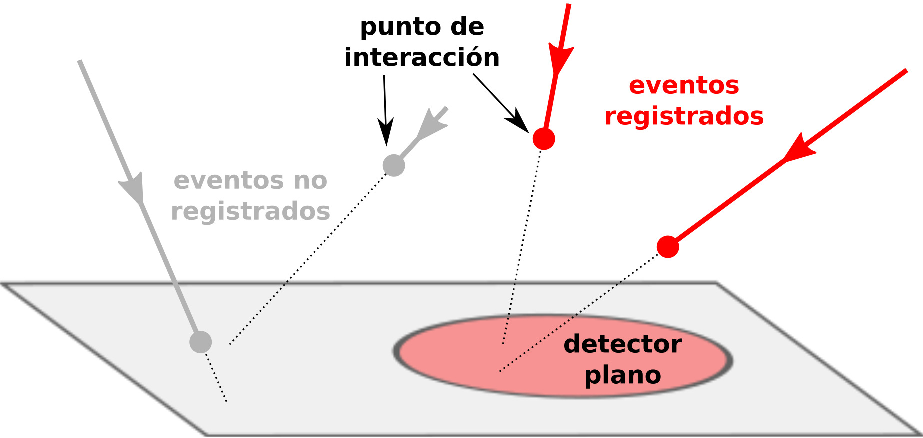
\includegraphics [width=0.52\textwidth]{fig/resultadosAuger/detectorPlano.pdf} & 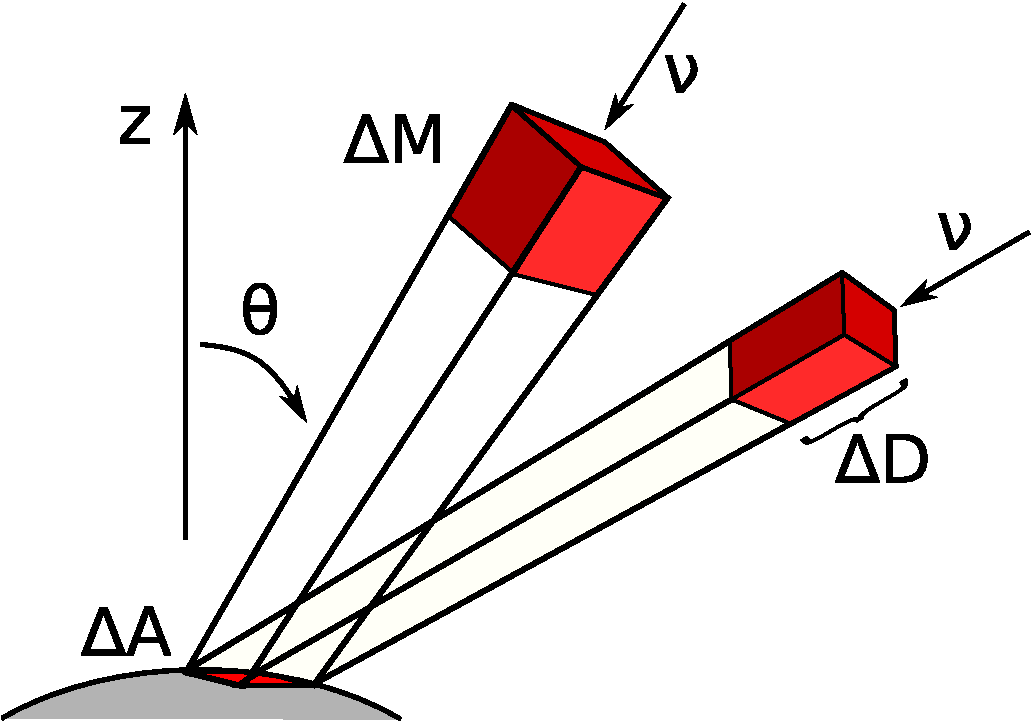
\includegraphics [width=0.42\textwidth]{fig/resultadosAuger/diferencialMasa.pdf}
	\end{array}$
	\end{center}
	\caption{
	\textit{Panel izquierdo}: vista esquemática de un detector plano imaginario que registra todos los eventos producidos por partículas cuya dirección de arribo cruza su superficie. \textit{Panel derecho}: diagrama de diferencial de masa $\Delta M$ según se define en el texto. Puede observarse que $\Delta M$ crece al disminuir el ángulo cenital $\theta$.
	}
	\label{fig:diferencialMasa}
	\end{figure}
	%
	
	Si el detector tiene una eficiencia~$\epsilon$ menor que uno, sólo una fracción de las lluvias serán detectadas. En el caso más general~$\epsilon$ es función de $E_{\nu}$, $\theta$, $D$, $\vec{r}$ y $\phi$:
	%
	\begin{equation}
	n = \frac{1}{m}\,\Phi(E_{\nu})\,\sigma(E_{\nu})\,\Delta E_{\nu}\,\Delta D\,\Delta A\,\cos\theta\sen\theta\,\Delta\theta\,\Delta\phi\;\epsilon(E_{\nu},\theta,D,\vec{r},\phi)
	\label{eq:dN_domega}
	\end{equation}
	%
	Integrando en $\phi$ tenemos:
	%
	\begin{equation}
	n = \frac{1}{m}\,\Phi(E_{\nu})\,\sigma(E_{\nu})\,\Delta E_{\nu}\,\Delta D\,\Delta A\,\cos\theta\sen\theta\,\Delta\theta\,2\pi\;\epsilon(E_{\nu},\theta,D,\vec{r})
	\label{eq:dN_domega2}
	\end{equation}
	%
	donde $\epsilon(E_{\nu},\theta,D,\vec{r}) = \frac{1}{2\pi}\int \epsilon(E_{\nu},\theta,D,\vec{r},\phi)\,\d\phi$ es el promedio de la eficiencia respecto del ángulo azimutal. 

	Si se mide durante un tiempo $T$, sumando las contribuciones de todos los bines, pasando a forma integral y reacomodando la ecuación \ref{eq:dN_domega2} se obtiene:
	%
	\begin{equation}
	N = \int\limits_{E_\nu}\Phi(E_{\nu})~
	\tilde{\cal E}_{DG}(E_{\nu})
	~dE_\nu
	\label{eq:dN_domega3}
	\end{equation}
	%
	donde:
	%
	\begin{equation}
	\tilde{\cal E}_{DG}(E_{\nu})
	\equiv 2\pi\iint\limits_{D~\theta}\frac{1}{m}~\sigma(E_{\nu})\cos\theta
		\left[
			~\iint\limits_{T~A} \epsilon(E_{\nu},\theta,D,A)~dA~dT
		\right]
		\sen\theta~d\theta~dD
	\label{eq:dN_domega4}
	\end{equation}
	
	Por otro lado, si se desarrolla el término $d\Omega$ y se integra en $\phi$ en la ecuación \ref{eq:exp4DG} se obtiene:
	\begin{equation}
	{\cal E}_{DG}(E_\nu)\equiv2\pi\iint\limits_{D~\theta}P(D|E_{\nu},\theta)~
	 \left[~
	 \iint\limits_{T~A}\epsilon(D,E_{\nu},A,\theta,T)~dA~dT
	 \right]
	 \sen\theta~d\theta~dD
	\label{eq:exp5DG}
	\end{equation}
	
	Entonces, por comparación entre \ref{eq:dN_domega4} y \ref{eq:exp5DG} se tiene como se esperaba, que $P(D|E_{\nu},\theta)$ es una constante y vale:
	\begin{equation}
	 P(D|E_{\nu},\theta) = \frac{1}{m}~\sigma(E_{\nu})\cos\theta
	\end{equation}
	
	En este trabajo se utilizó la sección eficaz neutrino nucleón dada en \cite{cite:cooper_sarkar}.
	
	\subsubsection{Eventos ES}
	
	La expresión de este término en el caso de los eventos ES es algo mas complicada debido a que el proceso de detección consta de dos pasos:
	\begin{enumerate}
	 \item La primer interacción dentro de la tierra y la propagación hasta el escape.
	 \item La propagación en la atmósfera hasta su decaimiento.
	\end{enumerate}
	
	En la sección \ref{sc:pesos} se analizó cada uno de estos pasos para corregir los pesos de las simulaciones de neutrinos ES.
	La inclusión de la propagación dentro de la tierra se realizó mediante simulaciones de montecarlo, como se detalló en la sección \ref{sbsbsc:sim_prop_tierra}.
	A partir de estas se obtuvo el término $f(E_\tau|E_\nu,\theta)$, que representa la densidad de probabilidad de la energía de los \tauon{}'s que escapande la tierra si los neutrinos incidentes tienen energía \enu{} y ángulo cenital $\theta$.
	Por otro lado, la incorporación de la probabilidad de decaimiento del \tauon{} en la atmósfera también se analizó en la sección \ref{sc:pesos} y esta dada por la ecuación:
	%
	\begin{equation}
		h(x_d,(E_\tau,\theta))=
		\exp{\left(
		-\frac{x_d}{|\cos\theta|\lambda(E_\tau)}
		\right)}
		\frac{1}{|\cos\theta|\lambda(E_\tau)}
	\end{equation}
	%
	Finalmente, es necesario incluir el término que tiene en cuenta la variación del diferencial de volumen en el que se produce la interacción con el ángulo cenital, $|\cos\theta|$.
	
	Con todo esto, desarrollando la integral en $\Omega$ e integrando en $\phi$ la ecuación \ref{eq:exp4ES} queda:
	%
	\begin{equation}
	\begin{aligned}
	 {\cal E}_{ES}(E_\nu)\equiv2\pi\iiint\limits_{E_\tau~{\rm x_d}~\theta}P({\rm x_d},E_\tau|E_{\nu},\theta)~
	 \left[~
	 \iint\limits_{T~A}\epsilon({\rm x_d},E_\tau,A,\theta,T)~dA~dT
	 \right]\\
	 ~\sen\theta d\theta~d{\rm x_d}~dE_\tau
	 \end{aligned}
	 \label{eq:exp5ES}
	\end{equation}
	%
	donde:
	\begin{equation}
	 P({\rm x_d},E_\tau|E_{\nu},\theta)=
	 f(E_\tau|E_\nu,\theta)
	 h(x_d,(E_\tau,\theta))
	 |\cos\theta|
	\end{equation}
	
	\subsection{Eficiencias de identificación en un detector infinito}
	\label{sbsc:idealEff}
	
	Para construir las eficiencias en un detector real es útil estidiarlas antes sobre un detector ideal.
	Mientras que el detector real no solo es finito sino que su forma puede variar en el tiempo, por ejemplo debido a que es común que las estaciones entren y salgan de servicio, un detector ideal consiste en una representación infinita y regular del verdadero.
	Entonces, para obtener las eficiencias de identificación de cada uno de los análisis se simuló una copia del SD de Auger de \cant{50\times50}{km}, infinita a los fines prácticos\footnote{Ningún eventos simulado supera los \cant{25}{km} de extensión.}, se lanzó sobre su centro lluvias simuladas y se obtuvo la señal en el detector tal como se explicó en la sección \ref{sc:offline}.
	Luego, se aplicaron los criterios de identificación de neutrinos desarrollados en el capítulo \ref{ch:selAuger} y se calculó la eficiencia en cada bin con la siguiente ecuación:
	%
	\begin{equation}
	 \epsilon_\chi(X)=\frac{N_{\chi}(X)}{N_{sim}(X)}
	 \label{eq:effDef}
	\end{equation}
	%
	donde $X$ es la etiqueta del bin, mientras que $N_{\chi}$ y $N_{sim}$ son la cantidad de lluvias que se identificaron con el criterio $\chi$ y simularon en el mismo. En nuestro análisis $\chi$ puede representar el nivel de disparo T3 del detector, la clasificación de  evento inclinado y la identificación como neutrino.
	
	\subsubsection{Eficiencias a neutrinos DG}
	
	La figura \ref{fig:effDG_tr_id} muestra la eficiencia de disparo T3 e identificación como función de la profundidad de interacción para lluvias iniciadas por $\nu_e$ via CC para \cant{10^{19}}{eV} y \cant{85}{^\circ}.
	%
	\begin{figure}[h!]
		\begin{center}
			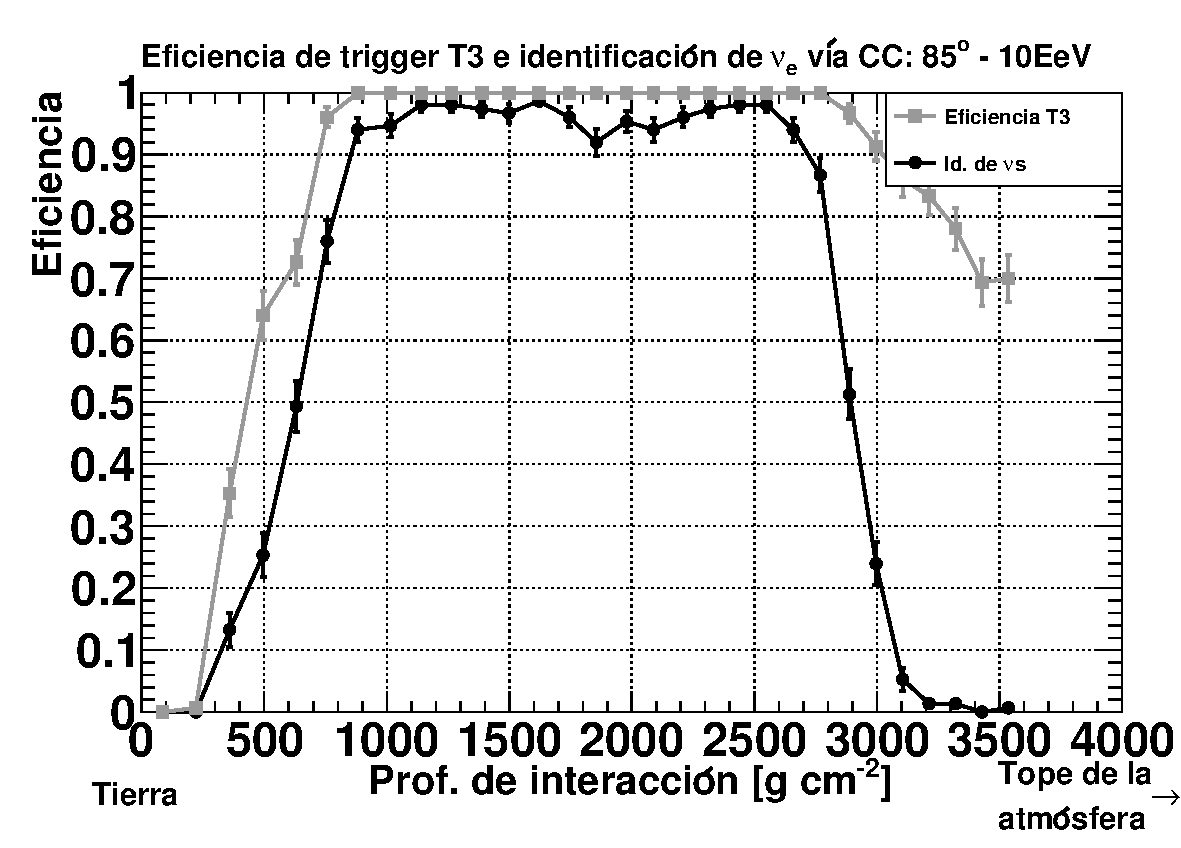
\includegraphics[width=0.7\textwidth]{fig/resultadosAuger/eff_10EeV_85}
			\caption{Eficiencia de disparo T3 e identificación en función de la profundidad de interacción para lluvias iniciadas por $\nu_e$ via CC con \cant{E_\nu=10^{19}}{eV} y \cant{\theta=85}{^\circ}}
			\label{fig:effDG_tr_id}
		\end{center}
	\end{figure} 
	%
	A esta energía y para este ángulo la eficiencia de disparo satura para profundidades intermedias.
	Cuando la lluvia se inicia muy cerca del detector no alcanza a evolucionar lateralmente lo suficiente como para disparar tres o mas estaciones, provocando menos eventos detectados. 
	Por otro lado, cuando se inicia alto en la atmósfera si bien en cerca del $70\%$ de los casos la componente muónica de la lluvia es suficiente para disparar el detector, no pueden ser identificados como neutrinos por ser muy similares a las lluvias iniciadas por hadrones.
	
	Por otro lado, en la figura \ref{fig:effDG_en} se muestran las eficiencias para lluvias iniciadas por $\nu_e$ via CC con \cant{\theta=85}{^\circ} y \cant{E_\nu=10^{17},~10^{18},~10^{19}}{eV}.
	Si bien, como era de esperarse\footnote{La cantidad de partículas que se genera con la lluvia son proporcionales a la energía de la misma.}, la eficiencia de detección disminuye con la energía del primario, las bajas energías son relativamente importantes en el cálculo de la exposición dado que los modelos actuales predicen una dependencia del tipo $E_\nu^{-2}$ para el espectro de energía de los neutrinos de origen cosmogénico.
	%
	\begin{figure}[h!]
		\begin{center}
			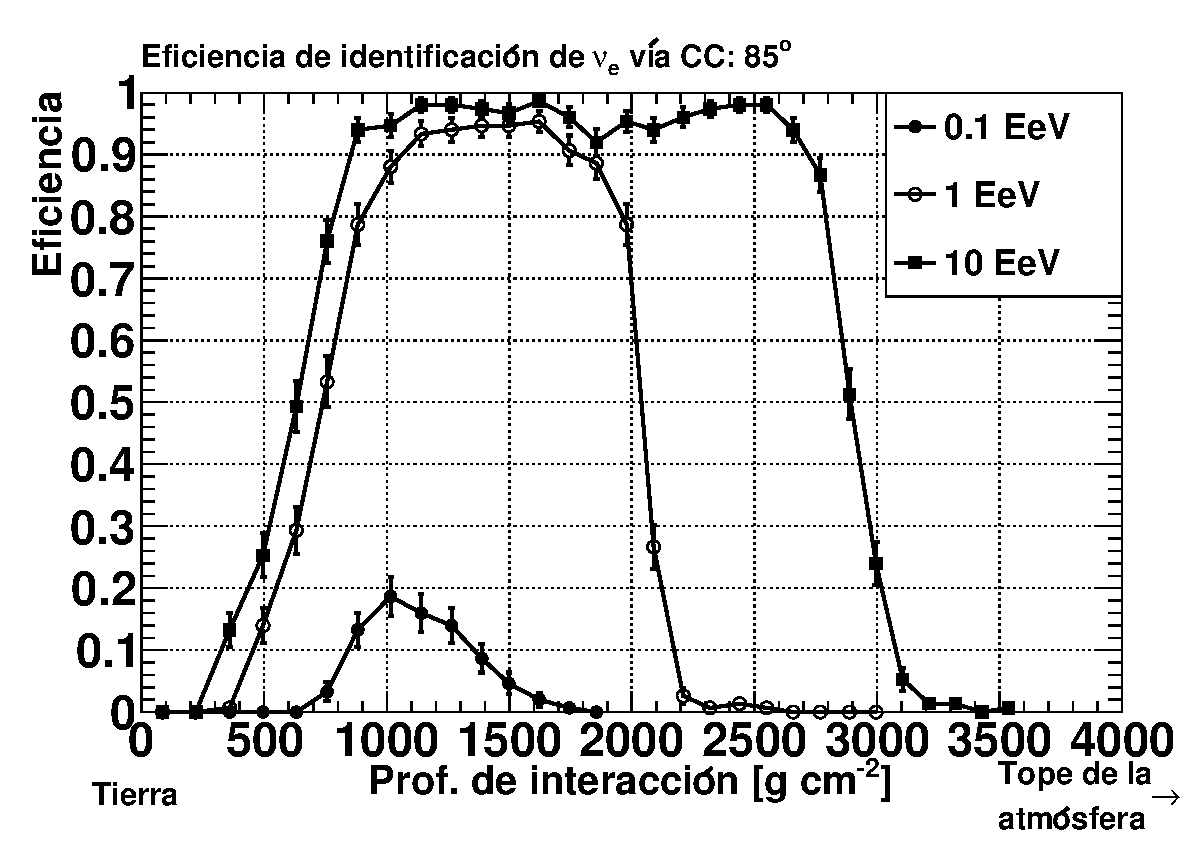
\includegraphics[width=0.7\textwidth]{fig/resultadosAuger/eff_varios_85}
			\caption{Eficiencia de identificación en función de la profundidad de interacción para lluvias iniciadas por $\nu_e$ via CC y por $\nu_x$ via CN para varias energías y \cant{\theta=85}{^\circ}}
			\label{fig:effDG_en}
		\end{center}
	\end{figure}
	%
	
	En la figura \ref{fig:effDG_th} se muestra como ejemplo las eficiencias de disparo e identificación para $\nu_e$ via CC y \cant{E_\nu=10^{18}}{eV} para \cant{\theta=80}{^\circ} en el panel izquierdo y para \cant{\theta=85}{^\circ} en el derecho.
	%
	\begin{figure}[h!]
		\begin{center}
			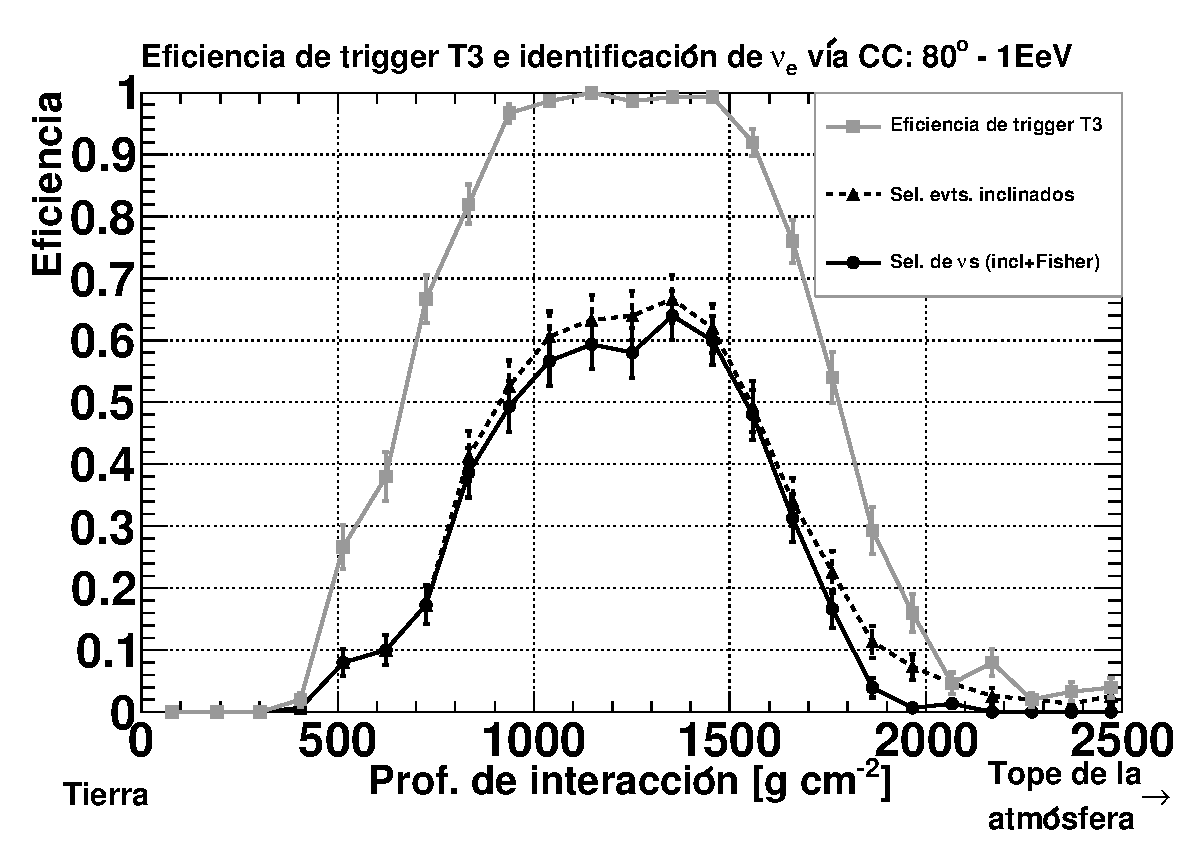
\includegraphics[width=0.47\textwidth]{fig/resultadosAuger/eff_1EeV_80}
			\hfill
			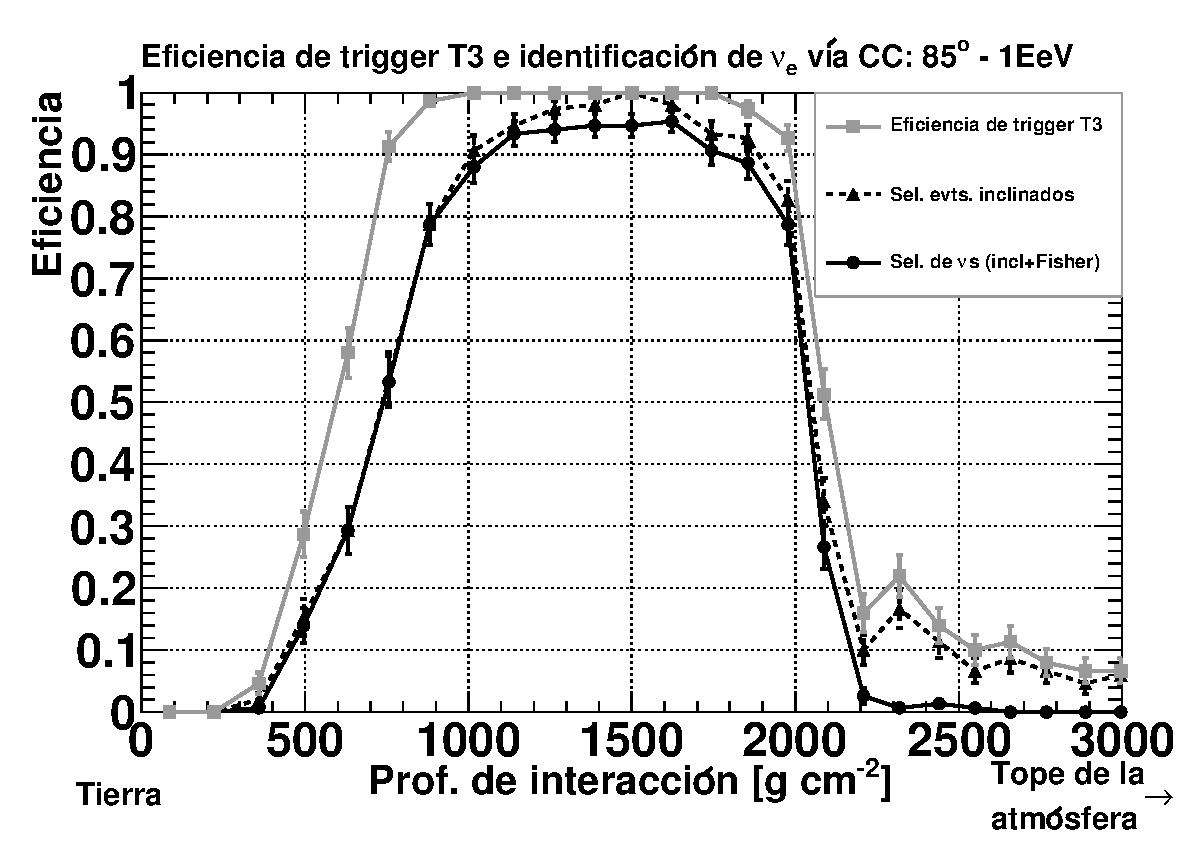
\includegraphics[width=0.47\textwidth]{fig/resultadosAuger/eff_1EeV_85}
			\caption{El panel izquierdo (derecho) muestra las eficiencias de disparo T3, de selección de eventos inclinados y de indentificación como función de la profundidad medida desde el detector para neutrinos con \cant{\theta=80}{^\circ} (\cant{\theta=85}{^\circ}). Es posible observar que la eficiencia alcanzada por el discriminante de fisher es alta para ambos ángulos.}
			\label{fig:effDG_th}
		\end{center}
	\end{figure}
	%
	En el panel izquierdo (\cant{\theta=80}{^\circ}) la eficiencia de disparo T3 alcanza el 100$\%$ a profundidades intermedias mientras que la eficiencia de identificación máxima es cercana a 60$\%$.
	Esta diferencia es producida por los cortes de selección de calidad, en los que para el canal DGH (al que corresponden estos ángulos) se requieren al menos 4 estaciones con disparo local T2, cuando el disparo global T3 requiere sólo 3.
	El panel derecho de la misma figura muestra las mismas eficiencias para \cant{\theta=85}{^\circ}, y se observa que la identificación alcanza valores cercanos a 95$\%$.
	Esta ganancia se debe a un efecto puramente geométrico, ya que la longitud de la huella sobre el detector crece con un factor aproximadamente $1/\cos\theta$, tal como se esquematiza en la figura \ref{fig:effDG_th_sktch}.
	%
	\begin{figure}[h!]
		\begin{center}
			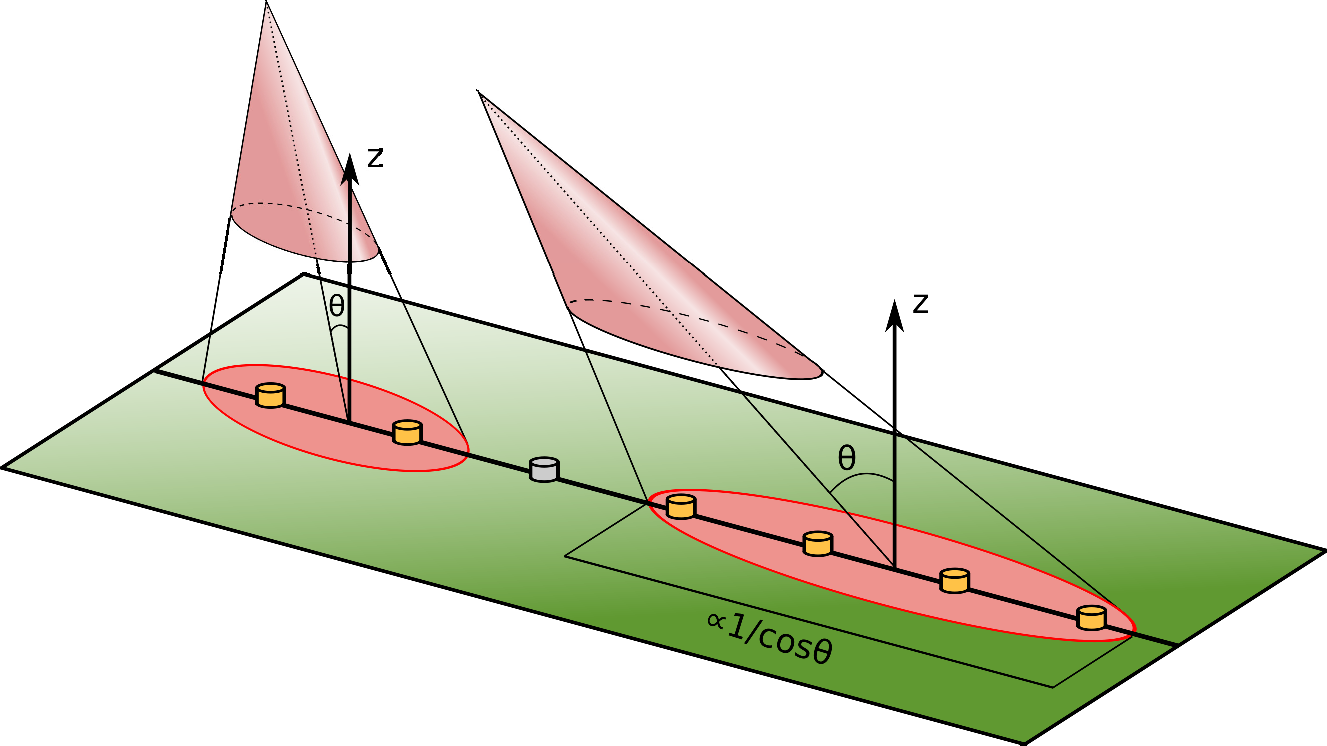
\includegraphics[width=0.7\textwidth]{fig/resultadosAuger/huellas}
			\caption{La cantidad promedio de estaciones disparadas por evento aumenta con el ángulo cenital $theta$ debido a que la huella de las llubias sobre el detector crece aproximadamente con un factor $1/\cos\theta$.}
			\label{fig:effDG_th_sktch}
		\end{center}
	\end{figure}
	%
	
	Otra particularidad de los neutrinos DG es que hay que hacer distinción entre los distintos sabores de neutrino y los canales de CC y CN.
	Dado que tanto en CN como en CC $\nu_\mu$ la energía transmitida a la lluvia es en promedio del 20$\%$ de la energía del neutrino, la eficiencia de estos canales será menor que el caso CC $\nu_e$, tal como se observa en el panel izquierdo de la figura \ref{fig:effDG_cc_nc}.
	%
	\begin{figure}[h!]
		\begin{center}
			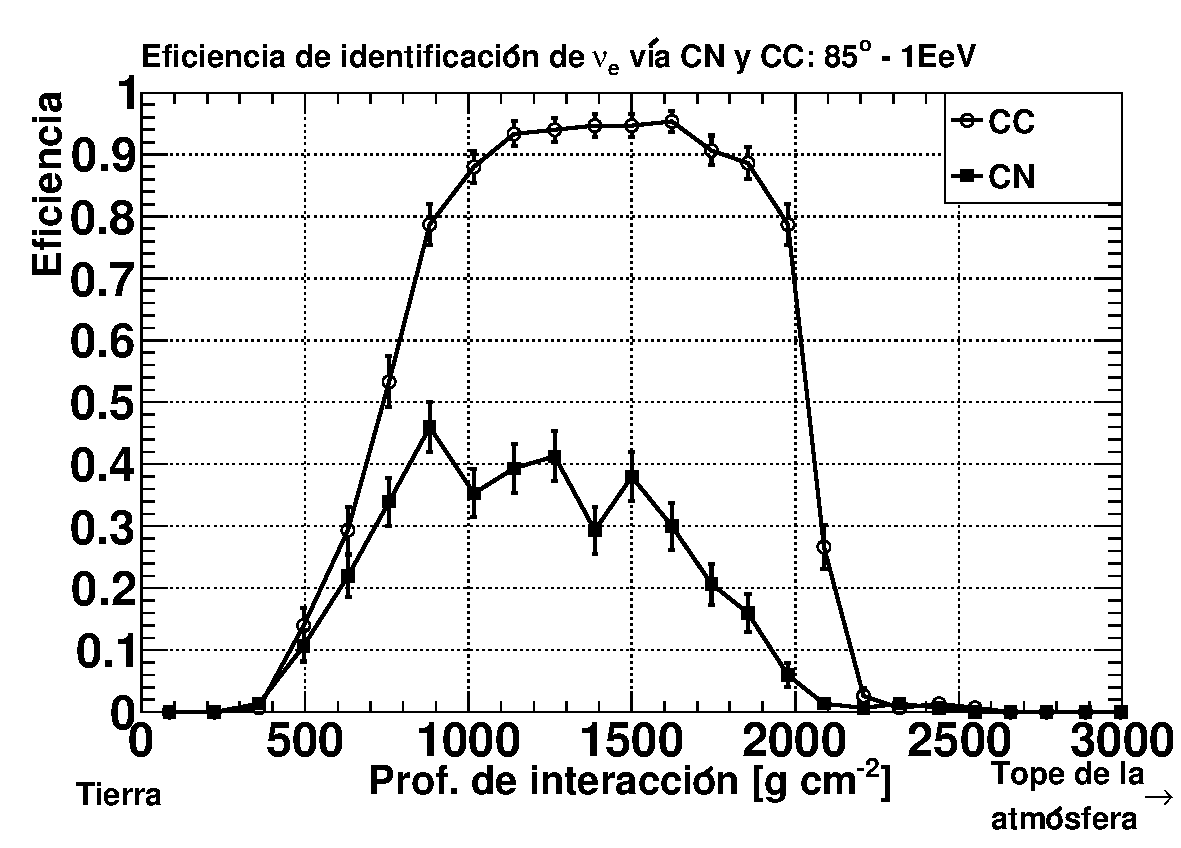
\includegraphics[width=0.47\textwidth]{fig/resultadosAuger/eff_CCvsNC_85}
			\hfill
			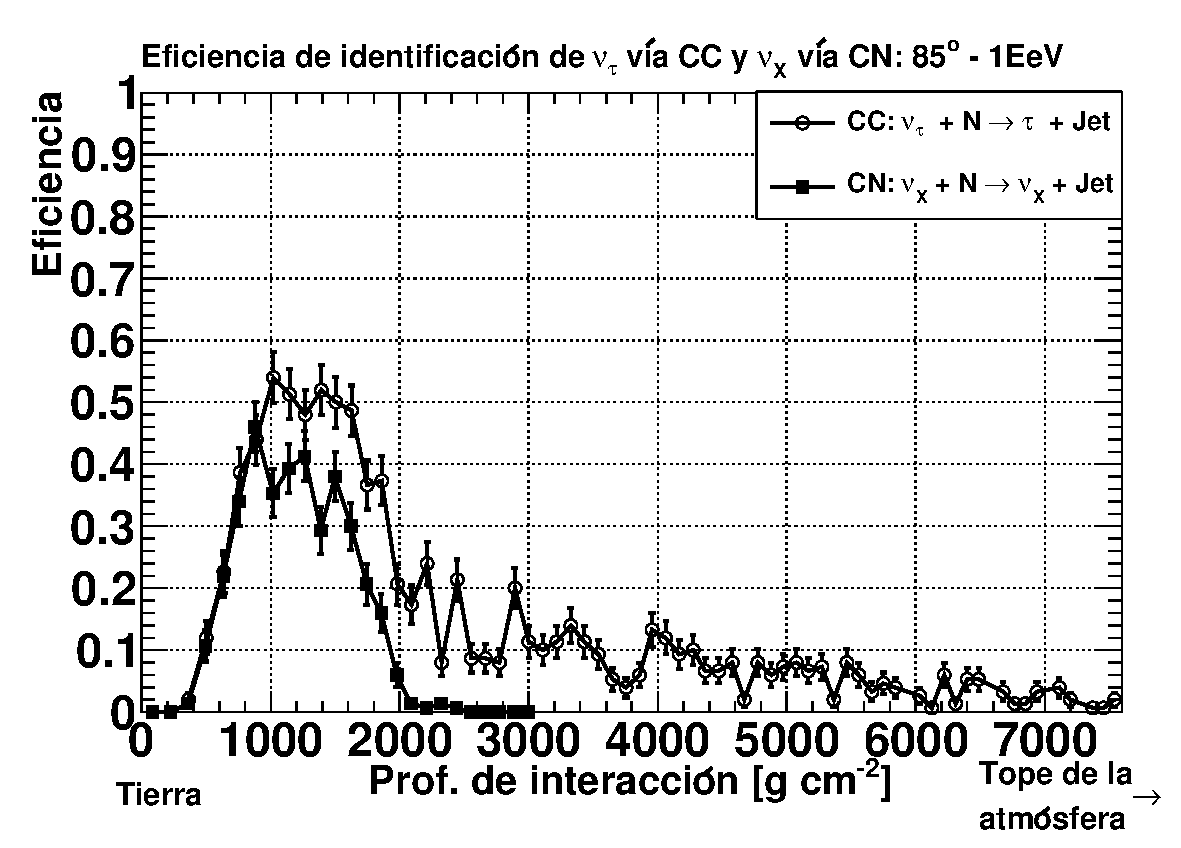
\includegraphics[width=0.47\textwidth]{fig/resultadosAuger/eff_tau_1EeV_85}
			\caption{Eficiencia de identificación en función de la profundidad de interacción para lluvias iniciadas por $\nu_e$ via CC y por $\nu_x$ via CN con \cant{10^{18}}{eV} y \cant{85}{^\circ}}
			\label{fig:effDG_cc_nc}
		\end{center}
	\end{figure}
	%
	El panel derecho de la misma se observa para los mismos parámetros la comparación entre el canal de CN y CC via $\nu_\tau$.
	En la sección \ref{sbsc:easDG} se explicó el mecanismo DB, en el que un $\nu_\tau$ interactua via CC produciendo un lepton $\tau$ que puede decaer generando una segunda lluvia a algunos km de la primer interacción.
	Teniendo en cuenta que la transferencia de energía $\nu$-nucleón no depende de si la interacción es via CC o CN, se deduce de la figura que incluso cuando la cascada generada en la primer interacción no es suficiente para disparar el detector (para profundidades mayores a \cant{\sim2000}{g cm^{-2}}) la segunda cascada a veces lo hace, recuperando del orden del 10$\%$ de los eventos.
	
	
	\subsubsection{Eficiencias a neutrinos ES}
	
	\subsection{Combinaci\'on de las eficiencias}
	
	\begin{figure}[h!]
		\begin{center}
			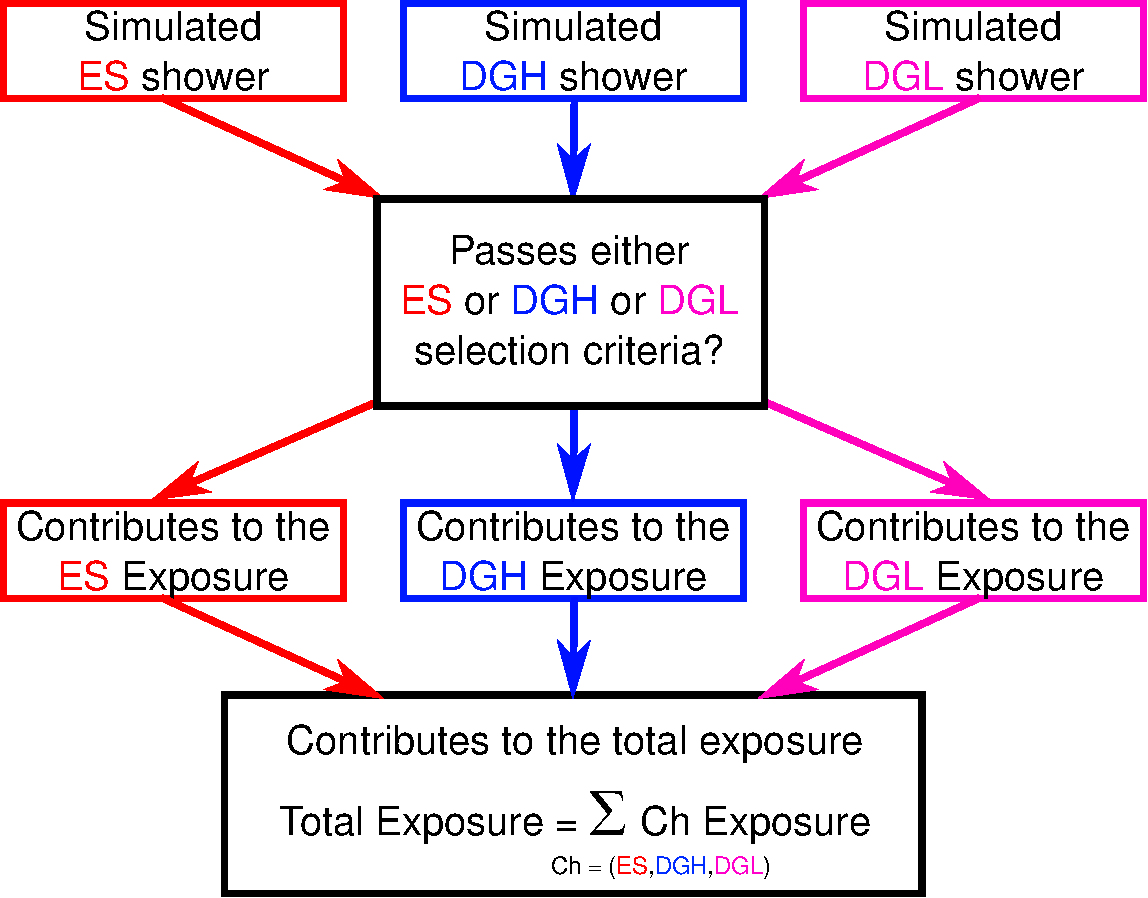
\includegraphics[width=0.9\textwidth]{fig/resultadosAuger/sketch_combined_4}
			\caption{asd}
			\label{fig:sketch_combined_4}
		\end{center}
	\end{figure}
	
% 	you are right, these numbers are important. I will work on that after the ICRC. For the moment I can only give you the exposure contribution (gain) in an E^{-2} scenario matrix, and it looks like:
% 
%           &    ES crit    &    DGH crit    &     DGL crit
% ES sh     &    0.695      &    0.035       &     neglect.
% DGH sh    &    0.045      &    0.185       &     neglect.
% DGL sh    &    neglect.   &    neglect.    &     0.04
% 
% please take into account that we have a systematic error of 40%. 
% for instance, from the table you can see that 3.5% of the total limit to an E^-2 flux is due to simulated 
% ES neutrinos selected by the DGH analysis. This gives an idea of the probability of "missclassification", but its no so simple, since the most of the ES simulated neutrinos that passes ES crit, also passes the DGH crit with a high reconstructed angle...
% In any case, if any of the three analysis finds a candidate we will have to scrutinize it with as many eyes 
% as possible and try to (1) make sure it is a neutrino and not a detector fluke, and (2) identify it as ES or 
% Down-Going quasi-horizontal, something that might not be that easy. 
	
	\subsection{Integración de las eficiencias sobre el área del detector}
	
	Para llevar a cabo la integración en área de la ecuación \ref{eq:exp2} es necesario estudiar cómo varían las eficiencias cuando se considera un detector finito, osea, con bordes.
	Cuando una lluvia cae sobre una región completamente instrumentada del detector (interior y sin estaciones faltantes) la eficiencia será la ideal, calculada en la sección \ref{sbsc:idealEff}.
	Por otro lado, existirán casos en los que parte de las partículas caen fuera del mísmo, como se esquematiza en la figura \ref{fig:lluviaFuera}, o en zonas con estaciones fuera de servicio.
	%
	\begin{figure}[h!]
		\begin{center}
			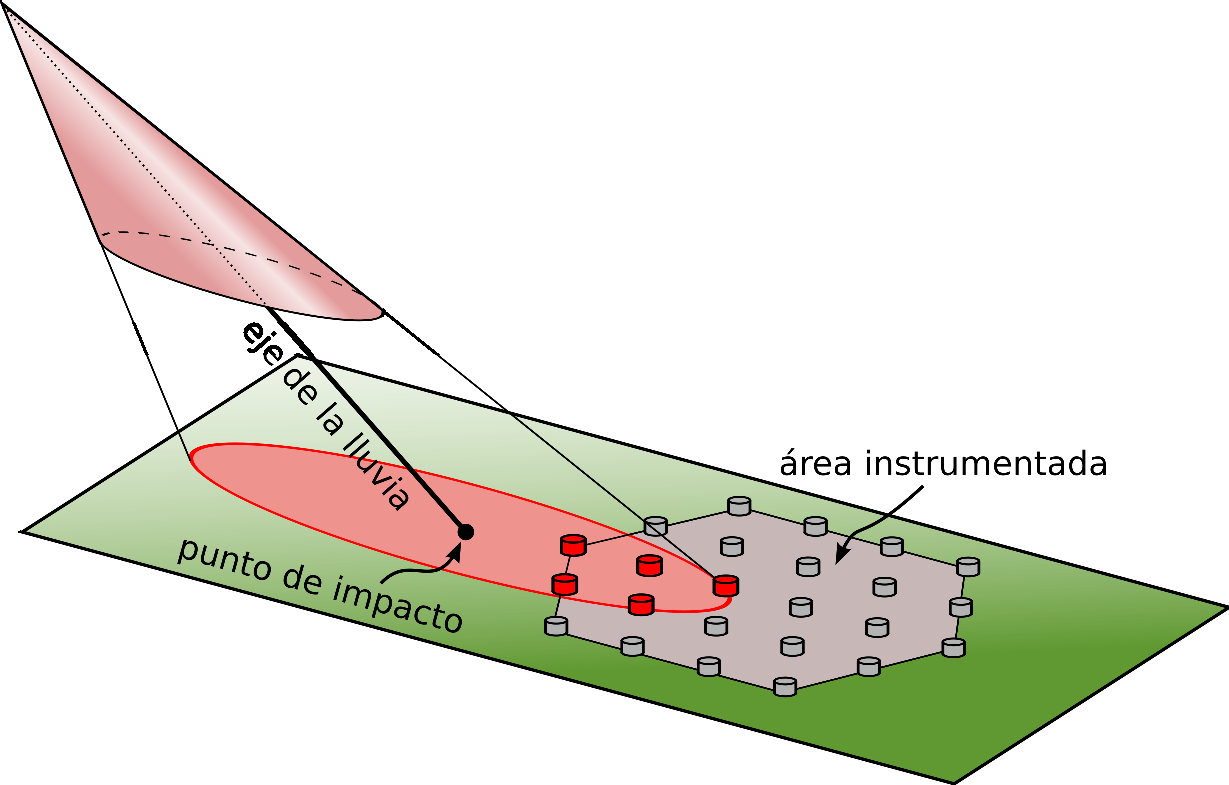
\includegraphics[width=0.9\textwidth]{fig/resultadosAuger/lluviaFuera}\\
			\vspace*{0.1\textwidth}
			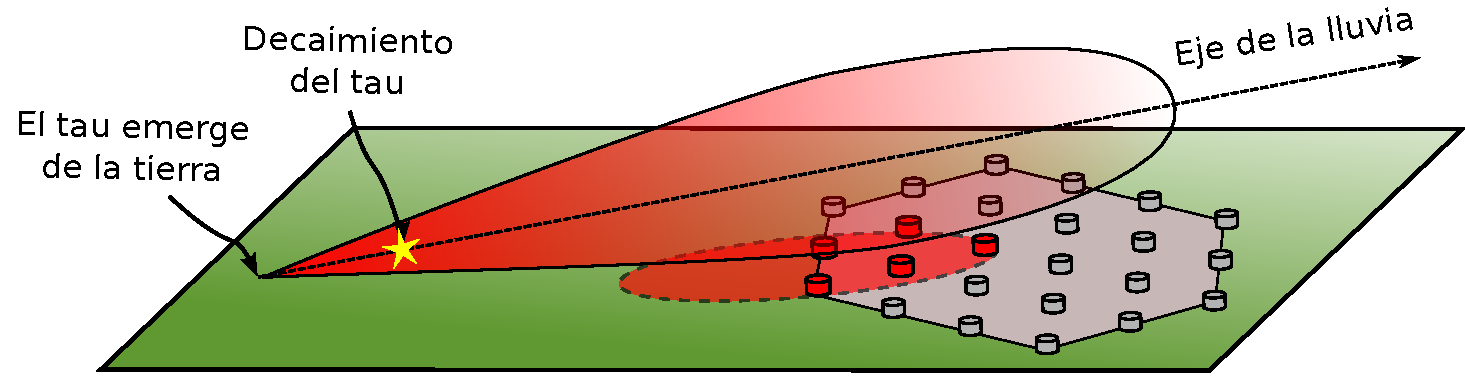
\includegraphics[width=0.9\textwidth]{fig/resultadosAuger/lluviaFuera_ES}
			\caption{asd}
			\label{fig:lluviaFuera}
		\end{center}
	\end{figure}
	%
	
	Bajo estas circunstancias, para evaluar las eficiencias de una configuración dada del detector es posible considerar un área extendida que contenga no sólo toda la región instrumentada, sino todas las ubicaciones de la huella de la lluvia que puedan disparar estaciones, lo que se puede observar en la figura \ref{fig:areaExtendida}.
	%
	\begin{figure}[h!]
		\begin{center}
			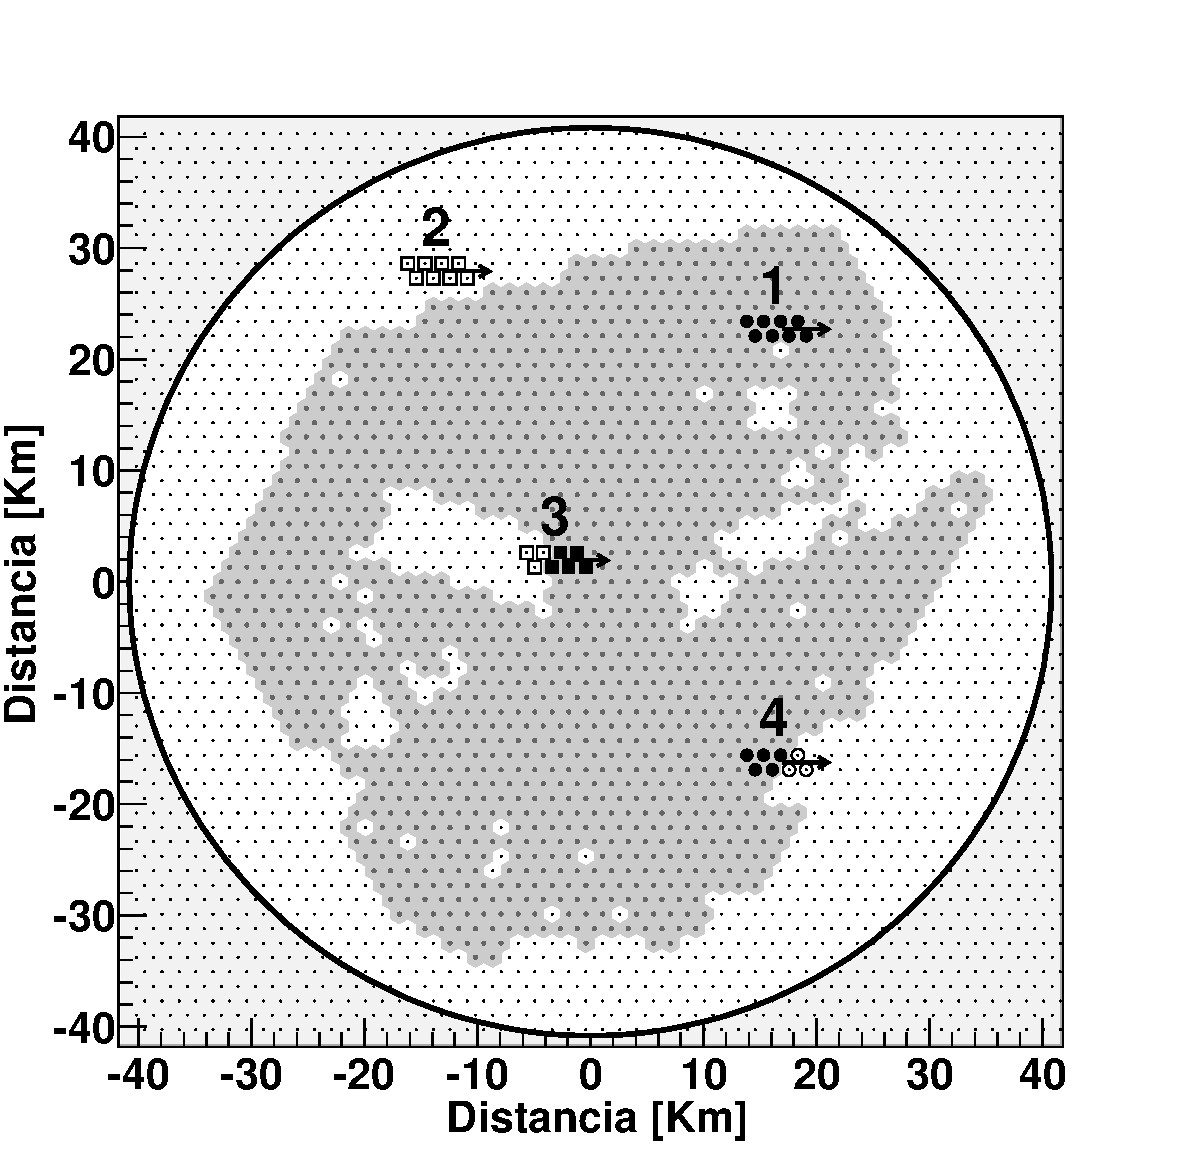
\includegraphics[width=0.9\textwidth]{fig/resultadosAuger/aperturaReal}
			\caption{asd}
			\label{fig:areaExtendida}
		\end{center}
	\end{figure}
	%
	
	Entonces, para realizar la integral en área de las eficiencias, 
	
	\subsection{Envejecimiento del detector}
	
	\begin{figure}[h!]
		\begin{center}
			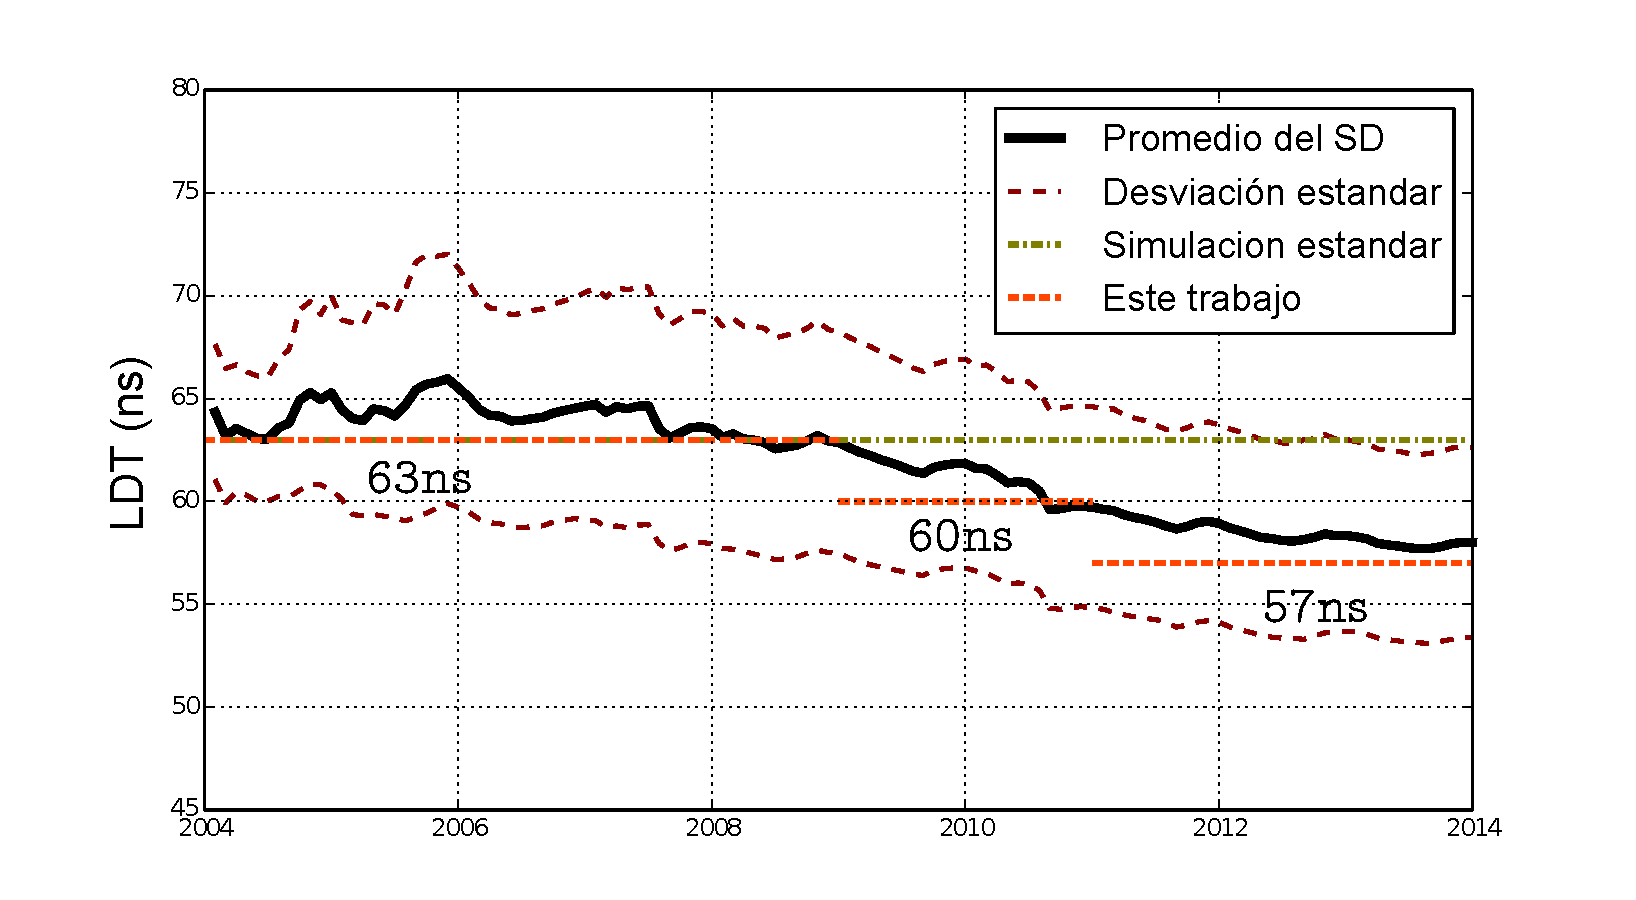
\includegraphics[width=\textwidth]{fig/resultadosAuger/timeEvolution}
			\caption{asd}
			\label{fig:}
		\end{center}
	\end{figure}
	
	\begin{figure}[h!]
		\begin{center}
			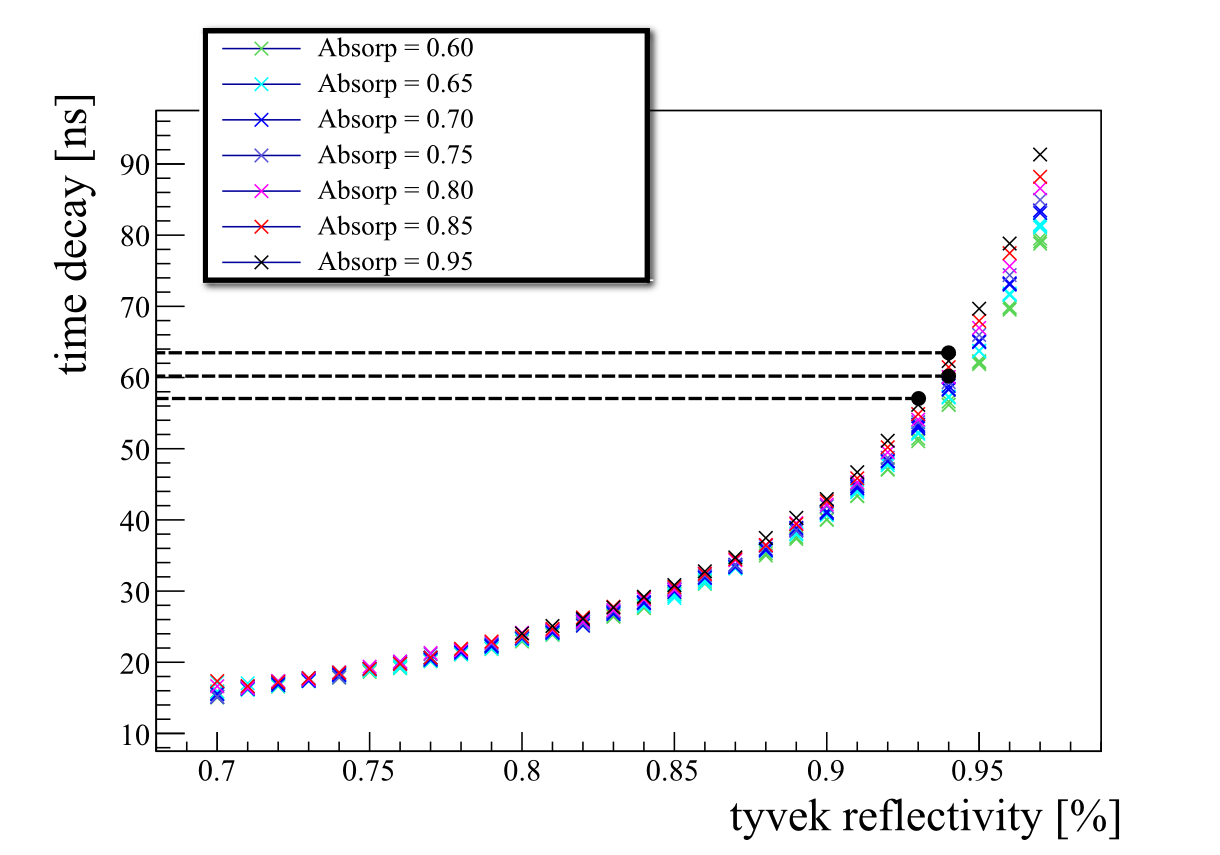
\includegraphics[width=0.9\textwidth]{fig/resultadosAuger/timedecay_vs_reflect_absorp}
			\caption{asd}
			\label{fig:}
		\end{center}
	\end{figure}
	
	\begin{figure}[h!]
		\begin{center}
			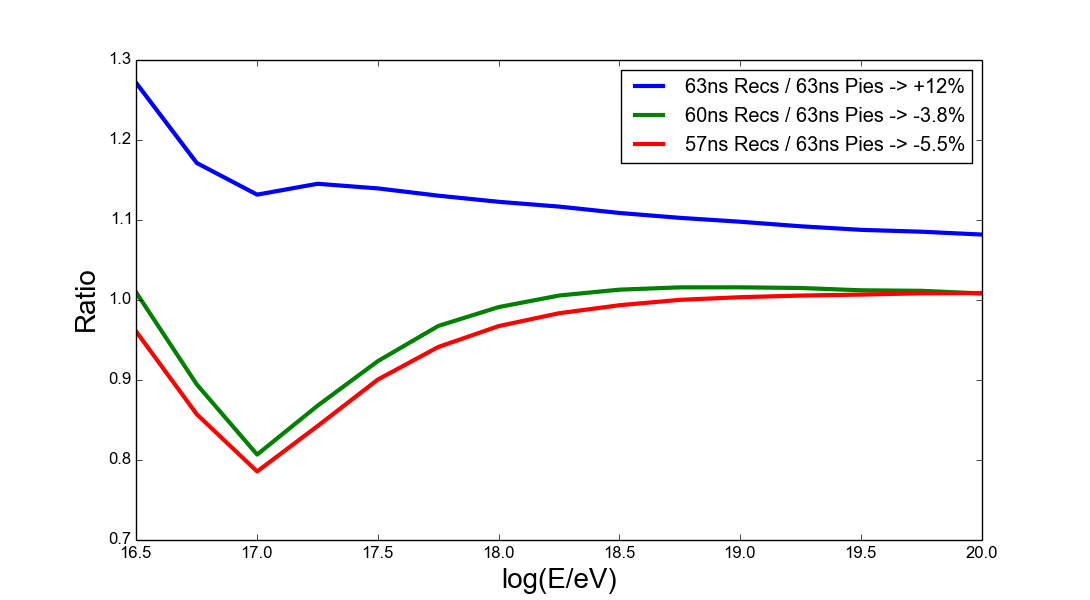
\includegraphics[width=0.9\textwidth]{fig/resultadosAuger/exposure_Arrays}
			\caption{asd}
			\label{fig:}
		\end{center}
	\end{figure}
	
	\begin{table}[h!]
	\centering
	\renewcommand{\arraystretch}{1.4}
	 \begin{tabular}{l|ccc|c|c}
				Período       & tyRef & wAbs & LDT        & Constribución &   Cambio relativo \\
				\hline
				$[2004 - 2008]$ & 0.94  & 100  & $\sim63$ns & $33.2\%$     &   $--$ \\
				$[2009 - 2010]$ & 0.94  & 80   & $\sim60$ns & $25.6\%$     &   $-15.2\%$\\
				$[2011 - 2013]$ & 0.93  & 100  & $\sim57$ns & $41.2\%$     &   $-17.5\%$\\
			\end{tabular}
	\end{table}
	
	\subsection{Integración temporal: evolución del detector}
	
	
	
	\subsection{Resultado final}
	
	\begin{figure}[h!]
		\begin{center}
			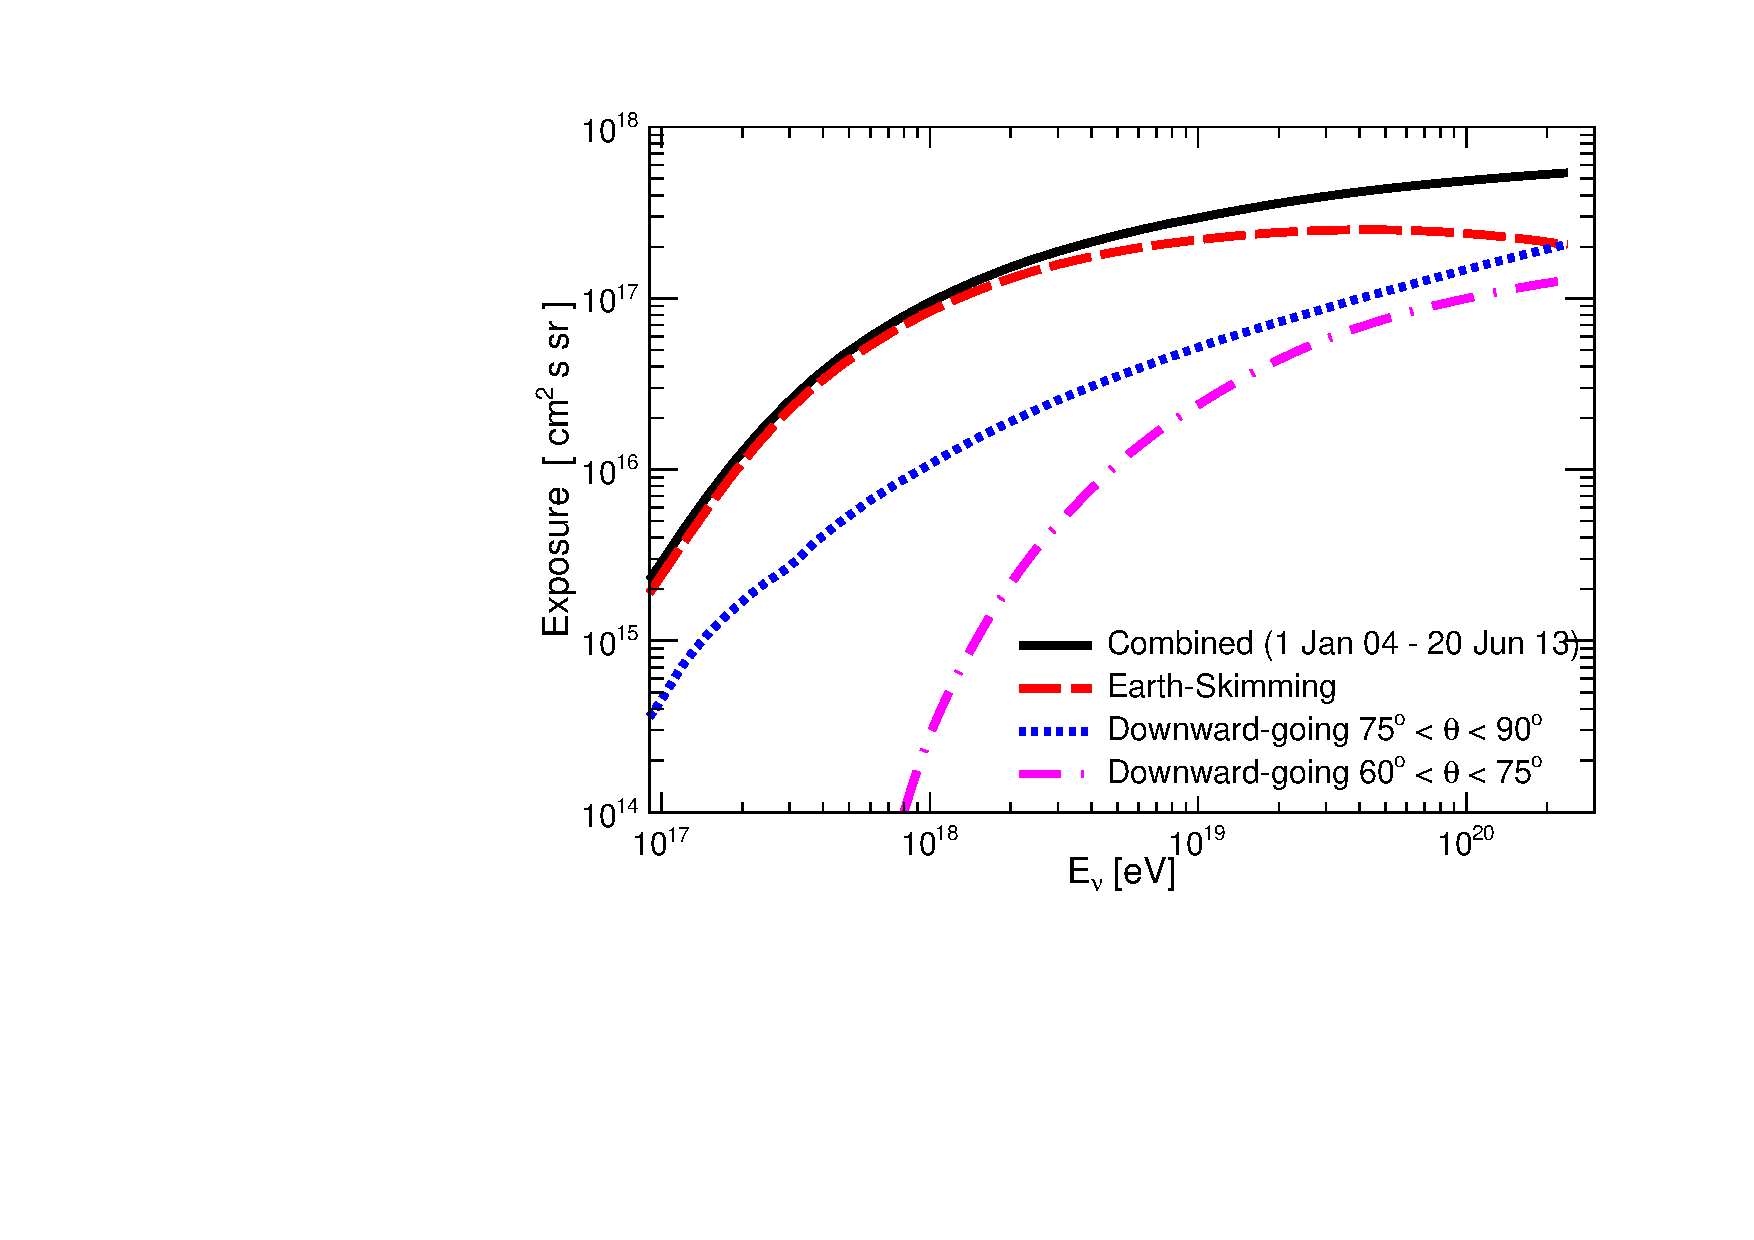
\includegraphics[width=0.9\textwidth]{fig/resultadosAuger/exposure_combined_ageing}
			\caption{asd}
			\label{fig:}
		\end{center}
	\end{figure}
	
\section{Errores sistem\'aticos}
			
	\begin{table}[h!]
	\centering
	\renewcommand{\arraystretch}{1.4}
	\footnotesize
		\begin{tabular}{|c|c|c|c|c|}
		\hline
		Source of  & ES        & DGH       & DGL        & Combined         \\
		systematic & ($90^\circ,95^\circ$) & ($75^\circ,90^\circ$) & ($65^\circ,75^\circ$) & ES / DGH / DGL   \\
		\hline
		& {\tiny \bf GAP 2013-100}     & \multirow{2}{*}{\tiny \bf PRD 84, 2011}    &   \multirow{2}{*}{\tiny \bf GAP2013-013} & \multirow{2}{*}{\tiny \bf 83.9\% / 13.7\% / 2.4\% }\\
		& {\tiny \bf PRD 79, 2009}     &     &  &  \\
		\hline
		
		Int. generator                   	    &  not eval.    &   0\%, -7\%     &   +3\%, -4\%  & +0.07\%, -1.0\% \\
		
		\hline
		
		pdf in generator                &  not eval.    &   0\%, -7\%     &   +4\%, -5\%  & +0.1\%, -1.0\% \\
		
		\hline
		
		EAS simulation	                     	    &  not eval. &   0\%, -17\%    &   +17\%, 0\%  & +0.4\%, -2.3\% \\
		
		\hline
		
		Hadronic model                  		    & +4.7\%, -1\%      &  +5\%, -2\%     &   +0\%, -6\%  & +4.6\%, -1.3\% \\
		
		\hline
		Thinning                                        & +0.3\%, 0\%   &  +7\%,  0\%     &   +7\%,  0\%  & +1.1\%, -0.0\% \\
		\hline
		Detector simulator                              & not eval.     &  not eval.      &   +5\%,  -5\% & +0.1\%, -0.1\% \\
		\hline
		\hline
		{\bf $\bm{ \sigma_{\nu_\tau}\ \otimes\ \tau}$ E-loss}    & \multirow{2}{*}{\textcolor{Red}{+40\%, -33\%}}  & \multirow{2}{*}{+9\%, -9\%}  & \multirow{2}{*}{+7\%, -7\%} & \multirow{2}{*}{\bf +33.6\%, -27.7} \\
		$\sqrt{H^2+I^2}$                                     &                 &                 &             & \\
		\hline
		\hline
% 				%%%%%%%%%%%%%%%%%%%%%%%%%%%%%%%%%%%%%%%%%%%%%%%%%%%%%%%%%%%%%%%%%%%%%%%%%%%%%%%%%%%%%%%%%%%%%%%%%%
		{\bf Topography} 	                            &  +18\%, 0\%    & included & not applicable   & +15.1\%, 0\%  \\

		\hline
		\hline
		{\bf Total}                     &  \multicolumn{3}{c|} {}  & {\bf +37.1\%, -27.9\%}         \\
		\hline
		%%%%%%%%%%%%%%%%%%%%%%%%%%%%%%%%%%%%%%%%%%%%%%%%%%%%%%%%%%%%%%%%%%%%%%%%%%%%%%%%%%%%%%%%%%%%%%%%%%
		\end{tabular}
	\end{table}

\section{Analisis ciego}

	\subsection{Abriendo la caja}
	
	\subsection{L\'imite al flujo difuso y diferencial}
	\begin{figure}[h!]
		\begin{center}
			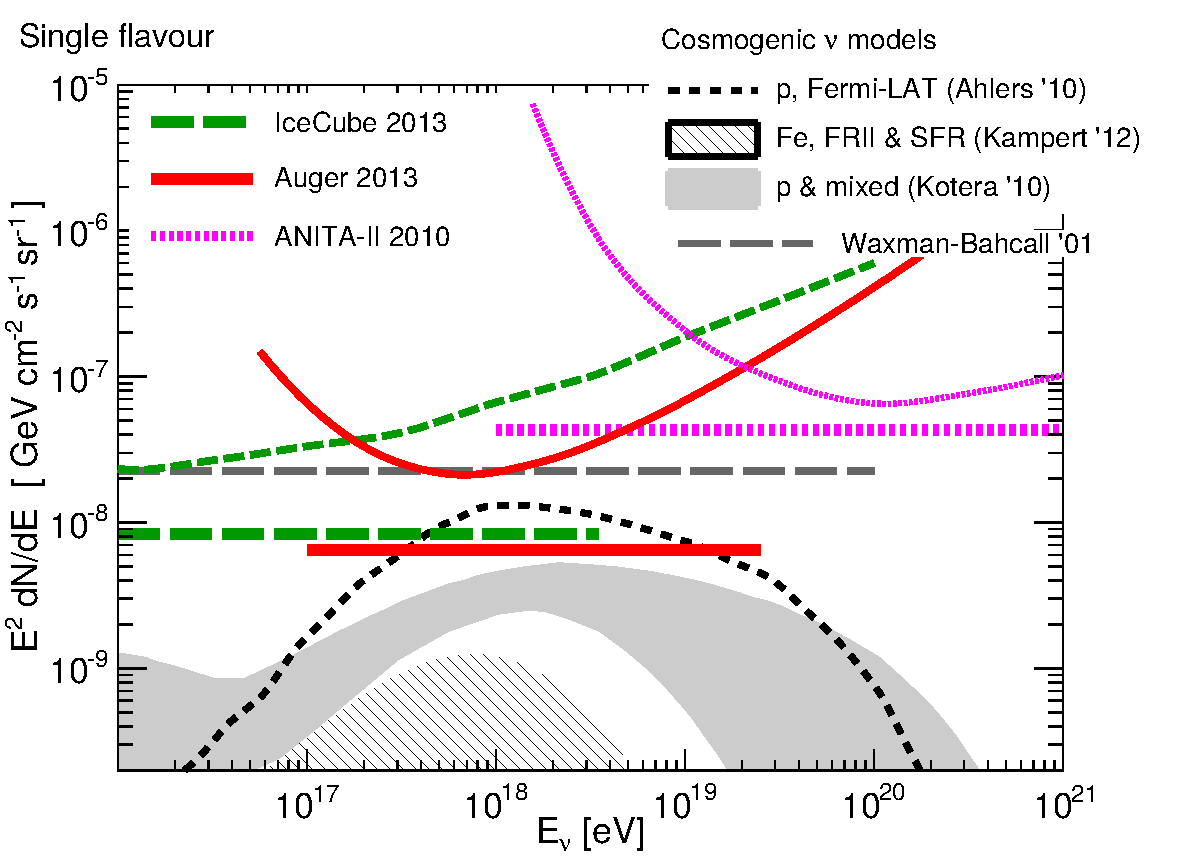
\includegraphics[width=0.9\textwidth]{fig/resultadosAuger/limits_combined_ageing}
			\caption{asd}
			\label{fig:}
		\end{center}
	\end{figure}
	
	\begin{table}[h!]
		\begin{center}
		\renewcommand{\arraystretch}{2.0}
			\begin{tabular}{|c|c|} 
			\hline
			Diffuse flux       &  Expected number of events   \\
			Neutrino Model     &  (1 Jan 04 - 20 Jun 13)   \\
			\hline
			\hline
			Cosmogenic (Kampert {\it et al.}) - proton, FRII      &  \textcolor{Red}{$\sim$ 4.0}  \\
			\hline
			Cosmogenic (Ahlers {\it et al.}) - proton, Fermi-LAT  &  \textcolor{Red}{$\sim$ 3.2}  \\
			\hline
			Cosmogenic (Kampert {\it et al.}) - proton, SFR       &  \textcolor{Blue}{$\sim$ 0.9}  \\
			\hline
			Cosmogenic (Kotera {\it et al.}) - band               &  \textcolor{Blue}{$\sim$ 0.5 $-$ 1.4}  \\
			\hline
			Cosmogenic (Kampert {\it et al.}) - iron, FRII        &  $\sim$ 0.3  \\
			\hline
			\end{tabular}
		\end{center}
	\end{table}
	

	
	\begin{figure}[h!]
		\begin{center}
			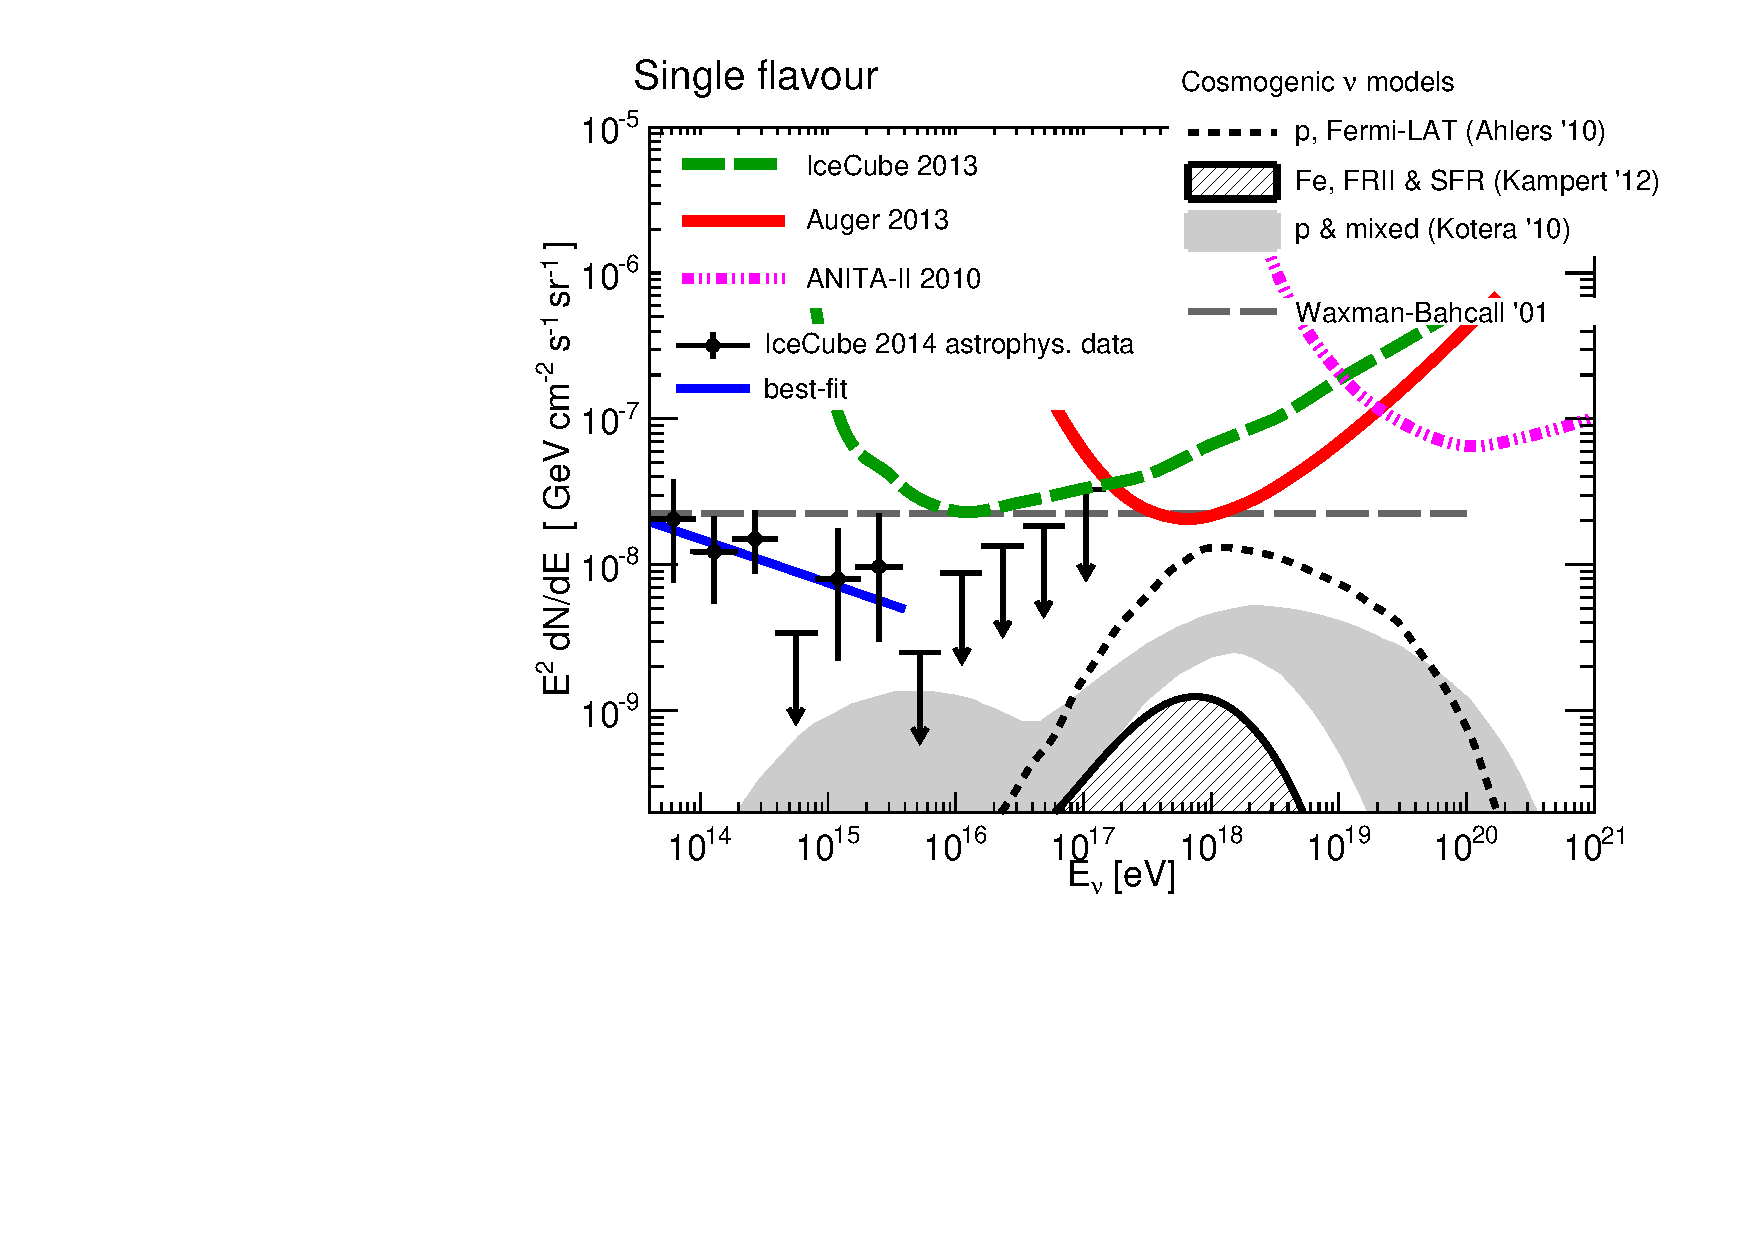
\includegraphics[width=0.9\textwidth]{fig/resultadosAuger/diff_limits_and_many_models_IceCube_data_noextrap}
			\caption{asd}
			\label{fig:}
		\end{center}
	\end{figure}

	
	